\documentclass[12pt]{article}
\usepackage[utf8]{inputenc}
\usepackage{array}
\newcolumntype{C}[1]{>{\centering\let\newline\\\arraybackslash\hspace{0pt}}m{#1}}
\usepackage[spanish]{babel}
 \usepackage{url}
\usepackage[spanish, fixlanguage]{babelbib}
\bibliographystyle{IEEEtran}
\usepackage{graphicx}
\graphicspath{ {./images/} }

\title{Paradigmas de programación Lógico y Funcional}

\author{
	Saul Ivan Rivas Vega \\
	Tarea 1\\
	Programación Avanzada\\
}

\date{\today}

\begin{document}
	\maketitle
	
	\section{Introducción}
	Una definición para el paradigma de programación es la interrelación entre algoritmos y datos, y que esta ha estado en constante evolución~\cite{joyanes_aguilar_fundamentos_2008} y esto se ha visto reflejado en la creación de nuevos paradigmas encontrando nuevas formas de ver esa interrelación dependiendo del caso de uso.
	\paragraph{}
	Es también una forma o estilo de programar, algunos lenguajes tendrán entonces una mayor facilidad  de escribir en ciertos paradigmas que otros.~\cite{loyola_university}
	\paragraph{}
	En este trabajo se hablará de los paradigmas lógico y funcional mencionando sus principales características, ventajas y desventajas así como los mas conocidos lenguajes que los representan.
	\section{Desarrollo}\label{desarrollo}
	
	
	\subsection{Paradigma Funcional}
	\subsubsection{Características}
	\paragraph{}
	En el paradigma funcional el programa principal es una función que recibe los parámetros de entrada como argumento y devuelve el resultado como salida, este programa principal esta compuesto de funciones y estas a su vez están compuestas de mas funciones quedando en el mas bajo nivel de definición los valores primitivos del lenguaje. ~\cite{why_functional}.
	\paragraph{}
	Estas funciones también deben ser puras, esto quiere decir que las funciones solo dependen de sus argumentos, sin hacer referencia o uso de variables en el entorno global, ademas de que no debe haber efectos secundarios, para preservar la inmutabilidad de las variables y el cambio de estado que influya en la evaluación de la función. ~\cite{hack_fp}
	\paragraph{}
	Podemos entonces hablar en el caso práctico que una función en un programa para que pueda ser llamada pura debe contar con variables locales que almacenen el resultado de alguna operación realizada a un elemento de entrada, por ejemplo, una función que calcule el resultado de alguna operación aritmética a un número esta función debe cumplir con que:
	\begin{itemize}
		\item No debe hacer uso de valores fuera de la definición de la función.
		\item No debe modificar la variable que recibe como entrada.
	\end{itemize}
	Lo cual dejaría como opción crear una variable que contenga el resultado de la operación sobre el número, como una multiplicación por el valor de una constante definida en la función u otro valor que recibiera como argumento, y devolver dicha variable.
	\subsubsection{Metodologías}
	Mencionaremos algunos de los métodos que se usan en la programación funcional como es el caso de las funciones de orden superior, las cuales reciben otras funciones como parte de sus argumentos o devuelven como resultado otra función.~\cite{leandro_fp}.
	\paragraph{filter} 
	Se recibe una colección de datos y una función de filtrado como entrada  y devuelve una colección de datos que contiene a los elementos que cumplan con la función de filtrado.
	\paragraph{map} 
	Se recibe una colección de datos y una función de modificación como entrada  y devuelve una colección de datos que contiene el resultado de aplicar la función de modificación a cada elemento.
	\paragraph{reduce} 
	Se recibe una colección de elementos y una función de reducción como entrada  y devuelve un solo dato que es el resultado de combinar los elementos usando la función de reducción, por ejemplo la suma de todos los elementos.
	\subsubsection{Lenguajes}
	\paragraph{}
	Algunos de los mas populares lenguajes usados para el paradigma funcional son \textbf{Haskell}, \textbf{Scala}, \textbf{F\#} e incluso con base en las propiedades que se requieren se pueden considerar lenguajes como \textbf{Python}, \textbf{Javascript} y \textbf{C++11}.
	Ahora si consideramos las características definidas y las capacidades que han mejorado en los lenguajes de programación podemos entonces registrar que tanto cumplen con el paradigma funcional los lenguajes llegando a representaciones como en \ref{fig:fp_language_table}.
		\begin{figure}[h]
			\centering
			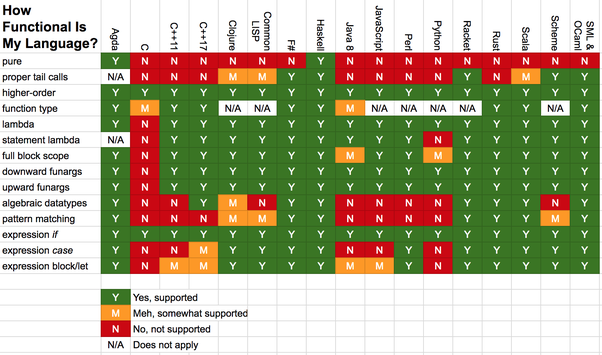
\includegraphics[width=1\textwidth]{fp_language_table}
			\caption{Características del paradigma funcional en los lenguajes de programación.~\cite{quora_fp}}
			\label{fig:fp_language_table} 
		\end{figure}
	\pagebreak
	\subsubsection{Ventajas y Desventajas}
	\paragraph{}
		\begin{table}[h!]
			\begin{center}
				\label{tab:fp_advantages_disadvantages}
				\begin{tabular}{|C{7cm} |C{7cm} |}
					\textbf{Ventajas} & \textbf{Desventajas} \\
					\hline
					El programa es mas expresivo al definir el programa con un enfoque  en que es lo que quiere lograr a diferencia de como lo quiere lograr. & Es mas complicado generar buen código estando influenciado por el predominante pensamiento imperativo.\\
					\hline
					Tiene una consideración en la seguridad con la inmutabilidad asegurándonos que una variable con un valor asignado no se alterará.& Las referencias de variables que solo contienen resultados parciales generan trabajo extra para el colector de basura.\\
					\hline
					El orden de ejecución de las funciones puede ser cambiado o incluso se puede llegar a aplicar paralelismo cuando no exista dependencia de datos entre dichas funciones. & Ciertos elementos inmutables como estructuras de datos que son mutables en lenguajes imperativos no siempre tienen un eficiente homologo en el paradigma funcional.\\
				\end{tabular}
			\caption{Ventajas y desventajas del paradigma funcional.}
			\end{center}
		\end{table}
	\subsubsection{Aplicaciones}
		\paragraph{}
		Se ha usado este paradigma en una serie variada de aplicaciones a nivel industrial y académico.
		La mayoría de estas se enfocan en el tratamiento de colecciones de datos, como es el caso de analizar métricas de rendimiento y poder realizar filtrados personalizados de una manera clara y concisa, otra razón por la cual es preferido para el tratamiento de datos en forma especifica es por el potencial de escalabilidad, al poder identificar fácilmente las dependencias entre las tareas o las que son independientes, lo que permite explotar los recursos de la computadora como los múltiples procesadores y paralizar la carga de trabajo alcanzando mayores velocidades.~\cite{testimonials_fs}
		\paragraph{}
		En la educación se utiliza mayormente por lo intuitivo que es definir una función matemática y poder pasar esa forma de abstracción a la programación permitiendo una enseñanza mas fluida en temas de programación y desarrollo en computación.
		
		
		
		
		
		\subsection{Paradigma Lógico}
		\subsubsection{Características}
		\paragraph{}
		En el paradigma lógico el programa esta escrito en un lenguaje lógico, el cual se diferencia de un lenguaje por que ademas de tener una sintaxis y una semántica tiene reglas de inferencia, haciendo que la ejecución del programa sea un proceso de validación de un teorema. En otras palabras las operaciones que realiza son inferencias lógicas.~\cite{introductioin_lp}.
		\paragraph{Sintaxis} Estas son las reglas que definen como escribir formulas lógicas.
		\paragraph{Semántica} Define el significado de las formulas en términos de consecuencias lógicas.
		\paragraph{Reglas de inferencia} Describen la forma correcta de llegar a una conclusión.
		\subsubsection{Metodologías}
		Algunos de los puntos que se deben enfatizar en el paradigma lógico para diferenciarlo de otros paradigmas son los siguientes:~\cite{DBLP:journals/corr/cs-PL-0107013}.
			\begin{itemize}
			\item Las operación se realizan en el dominio de todos los términos definidos en un alfabeto universal. 
			\item Los valores son asignados a variables en sustituciones generadas automáticamente llamadas \textit{unificadores generales}, dichos valores pueden contener variables llamadas \textit{variables lógicas}.
			\item El control es manejado por un solo mecanismo: \textit{backtracking automático}. Es decir que el control de flujo esta determinado por el seguimiento previo en las inferencias realizadas.
		\end{itemize}
				\pagebreak
	\paragraph{}Otras capacidades que tiene este paradigma son:
	\paragraph{Programación declarativa}  nos permite dar una \textit{interpretación de procedimientos}, la cual describe el como las operaciones son realizadas, y una \textit{interpretación declarativa} la cual describe el significado de que es lo que se esta computando. Lo cual permite entonces que al ejecutar un programa se esta ejecutando una especificación fácil de entender y desarrollar.
	\paragraph{Programación interactiva}  lo cual es que para un solo programa el usuario puede interactuar con el de distintas formas realizando preguntas que le son de interés. A lo cual si es necesario el desarrollador puede poner puntos de seguimiento en el ciclo de interacción.
		
		\subsubsection{Lenguajes}
		\paragraph{}
		Algunos de los lenguajes en el paradigma lógicos son~\cite{computer_hope}:

		\begin{list}{}{}
\item Absys
\item Alice
\item ASP (Answer Set Programming)
\item CycL
\item Datalog
\item Datomic
\item Logtalk
\item Mercury
\item Oz
\item Parlog
\item Planner
\item PROGOL
\item Prolog
	\end{list}
		
		\subsubsection{Ventajas y Desventajas}
		\paragraph{}
		\begin{table}[h!]
			\begin{center}
				\label{tab:lp_advantages_disadvantages}
				\begin{tabular}{|C{7cm} |C{7cm} |}
					\textbf{Ventajas} & \textbf{Desventajas} \\
					\hline
					Simple y conciso. & Uso de un solo mecanismo de control y un solo tipo de dato. (En algunos lenguajes puede modificarse) \\
					\hline
					Usos múltiples de un solo programa.& No tan eficiente como C.\\
					\hline
				El uso de backtracking puede ser de gran utilidad con problemas NP completos.& No ocupa un lugar reconocido por la industria a nivel de Java o C.\\
				\end{tabular}
				\caption{Ventajas y desventajas del paradigma lógico. ~\cite{DBLP:journals/corr/cs-PL-0107013}~\cite{introductioin_lp}}
			\end{center}
		\end{table}
		\subsubsection{Aplicaciones}
		\paragraph{}
		Mayormente las aplicaciones que tiene prolog son en el desarrollo de sistemas que interpretan otros lenguajes como el interprete del lenguaje Erlang, así como en el procesamiento de lenguaje natural, esto por la facilidad que tiene al parsear la entrada que en estos casos es un lenguaje completo. Una característica que se explota en sus aplicaciones es la de poder relacionar las reglas con consecuencias utilizadas en sistemas expertos con acceso a una gran base de conocimiento. Adicionalmente al tener soporte a multiples interacciones con un solo programa es utilizado en inteligencia artificial para la inferencia de tareas a realizar en un entorno cambiante. ~\cite{quora_lp}
		\section{Conclusiones}\label{conclusiones}
	El paradigma funcional y el paradigma lógico tienen casos de uso que hacen sus respectivos lenguajes que los representan una mejor selección que si seleccionaran algún otro con menos capacidades para las tareas a desarrollar. La información que respalde nuestras decisiones como desarrolladores debe estar fundamentada con una evaluación de lo que buscamos resolver y como esta puede beneficiarse de la mejor opción, si la definición del problema o la opción carece de beneficios al caso de uso el proyecto este será propenso de compensar sus carencias con complicaciones en el desarrollo. 
	\paragraph{}
	Los paradigmas mostrados en este trabajo son solo algunos de los que existen actualmente y de los que existirán en cuanto la interrelación entre algoritmos y datos evolucione con el tiempo dándonos la tarea de seguir evaluando y creando mejores soluciones que se adecuen a los retos actuales.
	
	
	\selectbiblanguage{spanish}
	\bibliography{main}
\end{document}